\documentclass[UTF8]{ctexart}
\usepackage{amsmath}
\usepackage{amssymb}
\usepackage{booktabs}
\usepackage{enumitem}
\usepackage{graphicx}

\title{决策理论 HW02}
\author{皇甫硕龙}

\newcommand{\N}{\mathbb N}
\newcommand{\R}{\mathbb R}
\newcommand{\Z}{\mathbb Z}
\newcommand{\C}{\mathbb C}
\newcommand{\dd}{\mathrm d}
\renewcommand{\geq}{\geqslant}
\renewcommand{\leq}{\leqslant}
\newcommand{\eqnref}[1]{(\ref{#1})}
\newcommand{\prob}[1]{P\left(#1\right)}
\newcommand{\cprob}[2]{P\left(#1|#2\right)}
\newcommand{\bs}{\boldsymbol}

\begin{document}
    \maketitle

    \paragraph*{1} 设计如下选项:

    \begin{enumerate}[label=\Alph*.]
        \item 获得(或损失)100元
        \item 以$x$的概率获得(或损失)$y$元
    \end{enumerate}

    设定概率$x$,通过访谈的方式测定当A、B等价时的收益(或损失)$y$,结果列于表\ref{tbl:result}(获得记为正,损失记为负)

    \begin{table}[ht]
        \centering
        \footnotesize
        \caption{实验结果}
        \begin{tabular}{ccc}
            \toprule
            概率$x$ & 收益$y$ & 损失$y$ \\
            \midrule
            $80\%$ & $+150$ & $-120$ \\
            $60\%$ & $+200$ & $-180$ \\
            $50\%$ & $+250$ & $-200$ \\
            $40\%$ & $+300$ & $-220$ \\
            $20\%$ & $+400$ & $-300$ \\
            \bottomrule
        \end{tabular}
        \label{tbl:result}
    \end{table}

    假设$u(100) = 100, u(-100) = -100$,当A、B等价时,效用函数满足$u(y) = u(100) / x$,则各个效用函数值列于表\ref{tbl:utility}

    \begin{table}[ht]
        \centering
        \footnotesize
        \caption{实验结果}
        \begin{tabular}{*{11}{c}}
            \toprule
            $y$ & $-300$ & $-220$ & $-200$ & $-180$ & $-120$ & $+150$ & $+200$ & $+250$ & $+300$ & $+400$ \\
            \midrule
            $u(y)$ & $-500$ & $-250$ & $-200$ & $-167$ & $-125$ & $+125$ & $+167$ & $+200$ & $+250$ & $+500$ \\
            \bottomrule
        \end{tabular}
        \label{tbl:utility}
    \end{table}

    曲线如图\ref{fig:curve}所示。

    \begin{figure}
        \centering
        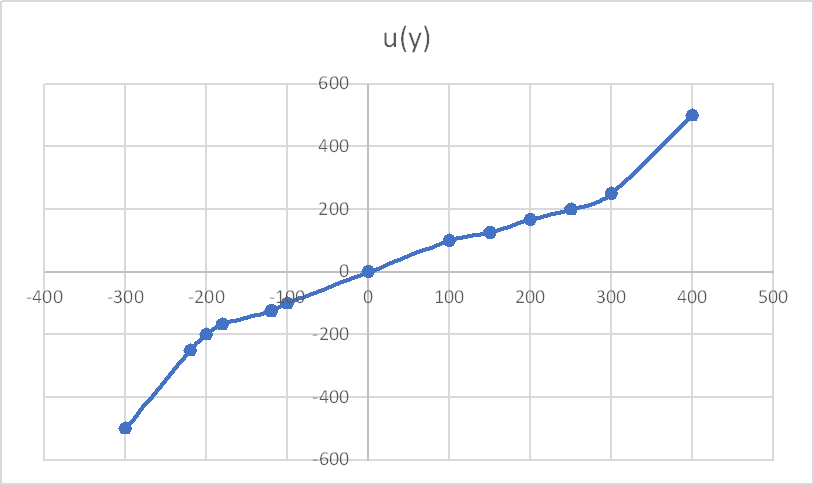
\includegraphics[height=5cm]{HW02-1.png}
        \caption{$y$-$u(y)$图}
        \label{fig:curve}
    \end{figure}

    使用三次函数进行拟合,结果为

    \begin{equation}
        u(y) = 6\times 10^{-6}y^3 - 0.0013y^2 + 0.6893y + 16.031
    \end{equation}

    风险类型为风险偏好型。

    \paragraph*{2} 设Jack的效用函数为$u(x)$,由于Jack在A、B中选择A,则有

    \begin{equation}
        u(1000) > 0.1u(5000) + 0.89u(1000)
        \label{eq:2-1}
    \end{equation}

    由于Jack在C、D中选择D,则有

    \begin{equation}
        0.11 u(1000) < 0.1u(5000)
        \label{eq:2-2}
    \end{equation}

    由\eqref{eq:2-1},有

    \begin{equation}
        0.11 u(1000) > 0.1u(5000)
    \end{equation}

    矛盾,因此不符合效用函数的假设。
\end{document}